% !TeX encoding = utf8
% !TeX spellcheck = en_US

\section{Results}
%\begin{table*}[ht]
%	\centering
%	\begin{tabular}{|l|c|c|c|c|c|c|c|}
%		\hline
%		\multirow{2}{*}{\textbf{Patient 563}} & \multicolumn{1}{c|}{\textbf{Mean $\pm$ Std}} & \multicolumn{6}{c|}{\textbf{Time in range [\%]}} \\ \cline{3-8}
%		&  & \textbf{(70-180)} & \textbf{(70-140)} & \textbf{(<70)} & \textbf{(<54)} & \textbf{(>180)} & \textbf{(>250)} \\ \hline
%		True                 & 153.4 $\pm$ 55.1    & 0.7    & 0.4    & 0.0    & 0.0    & 0.3    & 0.0    \\ \hline
%		Subsampling rate 1   & 153.4 $\pm$ 55.1    & 0.7    & 0.4    & 0.0    & 0.0    & 0.3    & 0.0    \\ \hline
%		Subsampling rate 2   & 153.4 $\pm$ 55.0    & 0.7    & 0.4    & 0.0    & 0.0    & 0.3    & 0.0    \\ \hline
%		Subsampling rate 4   & 153.3 $\pm$ 55.1    & 0.7    & 0.4    & 0.0    & 0.0    & 0.3    & 0.0    \\ \hline
%		Subsampling rate 8   & 153.8 $\pm$ 55.2    & 0.7    & 0.4    & 0.0    & 0.0    & 0.3    & 0.0    \\ \hline
%		Subsampling rate 16  & 153.0 $\pm$ 56.1    & 0.7    & 0.4    & 0.0    & 0.0    & 0.3    & 0.0    \\ \hline
%		Subsampling rate 32  & 152.3 $\pm$ 50.6    & 0.8    & 0.4    & 0.0    & 0.0    & 0.2    & 0.0    \\ \hline
%	\end{tabular}
%	\caption{Summary of the performance metrics for Patient 563 across different subsampling rates.}
%	\label{tab:patient563}
%\end{table*}
As shown in Figure \ref{fig:patients_mean}, the figure illustrates the mean blood glucose values (mg/dL) for each patient across various subsampling rates, ranging from the original resolution ("True") to the highest data reduction (subsampling rate 32). Each colored point represents the mean blood glucose value for an individual patient, with patients differentiated by color and labeled in the legend. Statistically significant differences between the subsampled mean values and the true mean values are indicated using asterisks, where $\ast \ast \ast = p \le 0.001$, $\ast \ast  = p \le 0.01$, and $\ast = p \le 0.05$.
The results show that the mean blood glucose values remain relatively consistent for lower subsampling rates (e.g., rates 1 and 2), but deviations become more pronounced at higher subsampling rates (e.g., rates 16 and 32). Statistically significant differences ($p \le 0.05$) are observed for several patients at these higher subsampling rates, as indicated by the presence of asterisks next to their corresponding data points. Notably, some patients (e.g., Patient 563 and Patient 559) show significant deviations even at intermediate subsampling rates, highlighting interindividual variability in the impact of data reduction.
\begin{figure}[h] % "ht" means "here" or "top", a positioning option
	\centering
	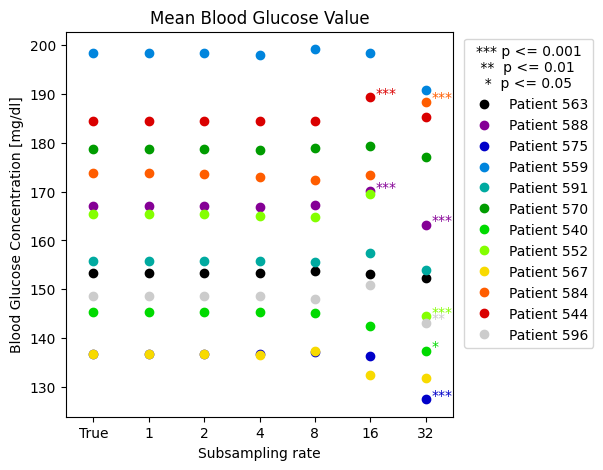
\includegraphics[width=\linewidth]{Figures/all_patients_mean_cbg_values.png} % Adjust the width as needed
	\caption{Mean blood glucose values across all patients in the dataset for various subsampling rates. The figure illustrates how the mean blood glucose value changes as the subsampling rate increases, highlighting the effect of reduced data resolution on the accuracy of the computed mean.}
	\label{fig:patients_mean}  % For referencing the figure in the text
\end{figure}

Furthermore, the results seen in Figure \ref{fig:patients_std} demonstrate that the standard deviation remains largely stable across lower subsampling rates (e.g., rates 1, 2, and 4). However, substantial reductions in standard deviation are observed at higher subsampling rates (e.g., rates 16 and 32), particularly for patients with higher baseline variability at the original resolution. This trend suggests that subsampling at extreme levels may suppress variability in the data, potentially masking important glucose fluctuations.
Up until an subsampling rate of 8 there appears to be a relatively low variability between the standard deviations.  In contrast, when the subsampling rate is increased to 16 and greater the  variability also increases drastically. 
\begin{figure}[h] % "ht" means "here" or "top", a positioning option
	\centering
	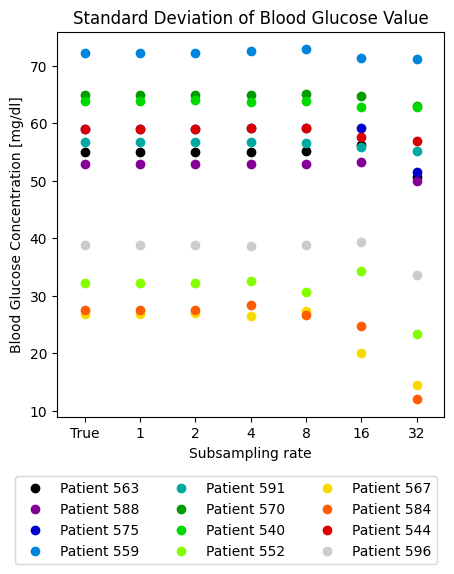
\includegraphics[width=\linewidth]{Figures/all_patients_std_cbg_values.png} % Adjust the width as needed
	\caption{Standard deviation of blood glucose values across all patients in the dataset for various subsampling rates. The figure illustrates how the standard deviation of blood glucose value changes as the subsampling rate increases, highlighting the effect of reduced data resolution on the accuracy of the computed standard deviaiton.}
	\label{fig:patients_std}  % For referencing the figure in the text
\end{figure}

Moreover, Figure \ref{fig:mses} presents the distribution of mean squared errors (MSEs) across various subsampling rates for blood glucose reconstruction. As depicted, the MSE remains relatively low and consistent for lower subsampling rates (1, 2, and 4), indicating minimal reconstruction error. However, as the subsampling rate increases, the MSE grows significantly, with a sharp rise observed at rates of 16 and 32. This trend reflects the loss of information and reduced accuracy of reconstruction as fewer data points are sampled. The widening distribution for higher subsampling rates, especially at rate 32, highlights greater variability in reconstruction error across patients.

\begin{figure}[h] % "ht" means "here" or "top", a positioning option
	\centering
	
\includegraphics[width=\linewidth]{Figures/distribution_mses.png} % Adjust the width as needed
	\caption{Distribution of Mean Squared Errors (MSEs) across subsampling rates for blood glucose reconstruction. MSE remains low at subsampling rates 1, 2, and 4, but increases sharply at rates 16 and 32, highlighting the trade-off between sampling frequency and reconstruction accuracy. Higher subsampling rates lead to greater variability and error in the reconstruction.}
	\label{fig:mses}  % For referencing the figure in the text
\end{figure}
Figure \ref{fig:mses_poly5} presents the distribution of mean squared errors (MSEs) for a degree-5 polynomial interpolation across various subsampling rates. At lower subsampling rates (e.g., rates 1, 2, and 4), the polynomial interpolation method exhibits higher MSEs compared to the cubic spline method, indicating reduced accuracy in reconstructing the true signal. However, at higher subsampling rates (e.g., 16 and 32), the performance of the polynomial method approaches that of the cubic spline, with comparable MSE values and variability. Since the cubic spline interpolation consistently demonstrated lower MSEs and superior performance overall, only its results are included in the main discussion.
\begin{figure}[h] % "ht" means "here" or "top", a positioning option
	\centering
	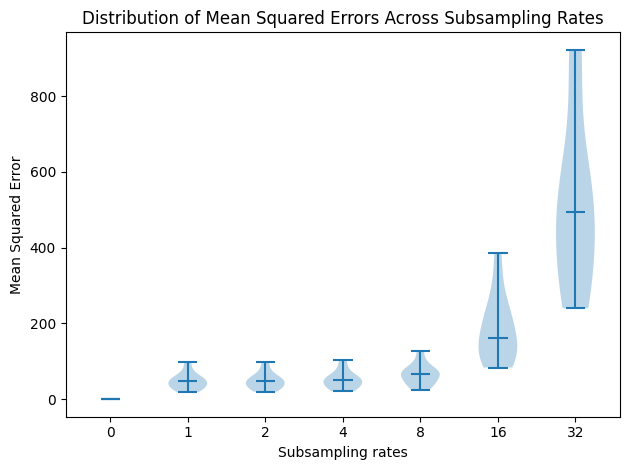
\includegraphics[width=\linewidth]{Figures/distribution_mses_poly5.png} % Adjust the width as needed
	\caption{Distribution of Mean Squared Errors (MSEs) across subsampling rates for blood glucose reconstruction with a polynomial of degree 5.}
	\label{fig:mses_poly5}  % For referencing the figure in the text
\end{figure}


Figure \ref{fig:SR_combined} shows that the reconstructed blood glucose signals demonstrate a clear decline in accuracy as the subsampling rate increases. At low subsampling rates (e.g., 1, 2 and 4), the reconstructed signals closely align with the true signal, indicating minimal information loss. However, as the subsampling rate increases to 8, 16, and 32, the reconstructions progressively deteriorate, deviating significantly from the true signal. This degradation is characterized by the smoothing or distortion of key features in the blood glucose dynamics, reflecting the impact of reduced sampling frequency on reconstruction fidelity. 
% These findings underscore the trade-off between sampling frequency and signal accuracy, emphasizing the limitations of high subsampling rates in preserving the integrity of glucose monitoring data.
\begin{figure*}[ht] % "ht" means "here" or "top", a positioning option
	\centering
	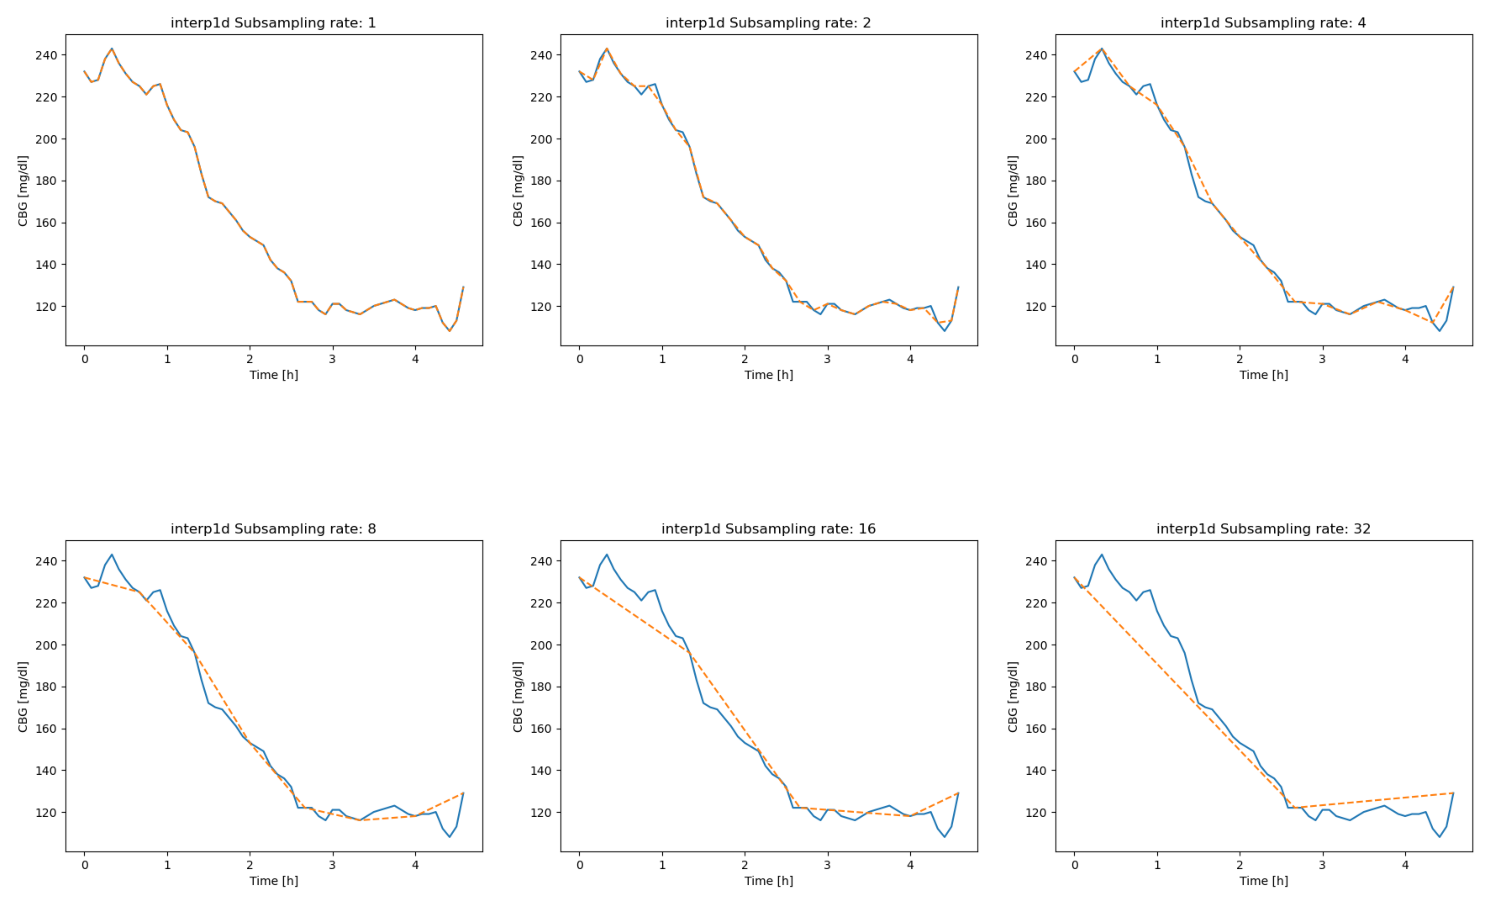
\includegraphics[width=\textwidth]{Figures/SR_combined.png} % Adjust the width as needed
	\caption{Subsampled reconstruction by cubic spline interpolation of the true signal for different subsampling rates. The figure shows a 2x3 grid of subplots where each plot represents the reconstructed signal from the true signal using various subsampling rates. The subsampling rates are 1, 2, 4, 8, 16, and 32, respectively, and are visualized to assess the impact of different levels of data reduction on signal fidelity. The red asterix shows the subsampled data points.}
	\label{fig:SR_combined}  % For referencing the figure in the text
\end{figure*}


Figure \ref{fig:time_in_ranges} shows the percentage of time spent in different blood glucose ranges - \textbf{Time in low (<70 mg/dL)}, \textbf{Time in range (70-180 mg/dL)},  and \textbf{Time in high (>180 mg/dL)} - for each patient under various subsampling rates, from the original resolution ("True") to the highest subsampling rate (32). 
\begin{itemize}
	\item \textbf{Time in Low (<70 mg/dL}: Across all subsampling rates, most patients maintain a low percentage of time spent in the hypoglycemic range, generally below 5\%. Subsampling does not significantly alter the time spent in this range for most patients. However, a small subset of patients (e.g., the green and yellow dots) exhibit higher percentages of time in hypoglycemia, with minimal variation across subsampling rates.
	\item \textbf{Time in Range (70-180 mg/dL)}: For the majority of patients, the percentage of time in the target range remains consistent across lower subsampling rates (rates 1, 2, and 4). At higher subsampling rates (16 and 32), minor deviations are observed for some patients. Notably, patients with consistently high percentages of time in range at the original resolution (e.g., the yellow and gray dots) maintain stability even under extreme subsampling. Conversely, patients with more variability at the original resolution exhibit slight decreases in time in range as subsampling increases.
	\item \textbf{Time in High (>180 mg/dL)}: The time spent in hyperglycemic ranges remains relatively stable across lower subsampling rates but shows a reduction at higher rates (16 and 32) for several patients. This is particularly evident for patients with a higher initial percentage of time in hyperglycemia (e.g., orange and blue dots), indicating that increased subsampling may underestimate time spent in elevated glucose levels.
\end{itemize}
% These results suggest that subsampling has minimal impact on time spent in different ranges for most patients at lower rates but begins to distort the representation of glucose dynamics at higher subsampling rates. This is especially true for patients with greater glycemic variability or those spending significant time in extreme glucose ranges.
\begin{figure*}[ht] % "ht" means "here" or "top", a positioning option
	\centering
	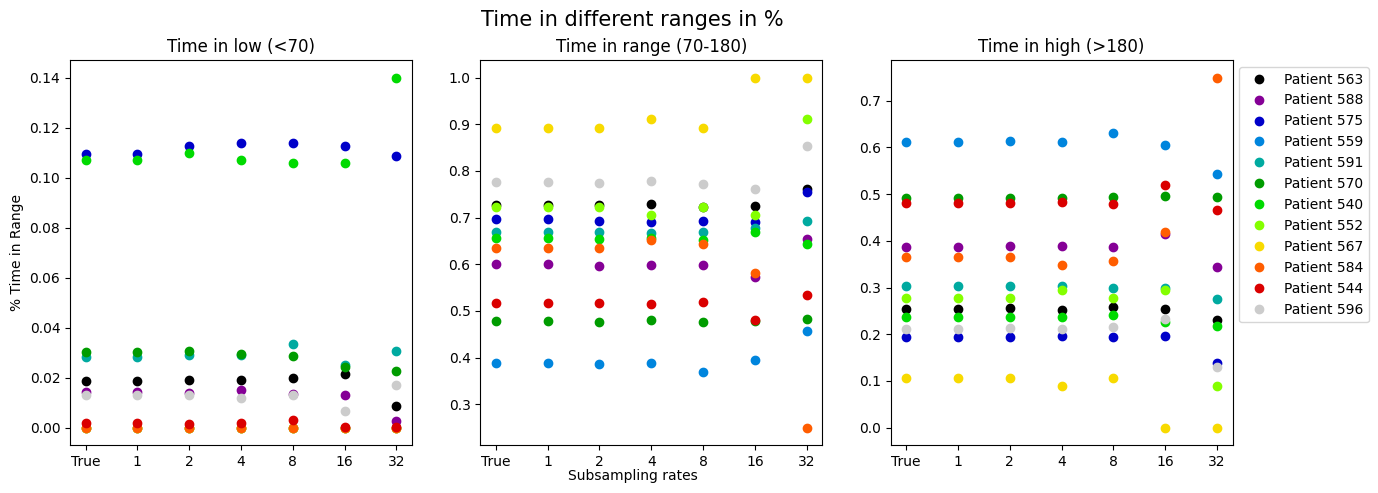
\includegraphics[width=\linewidth]{Figures/all_patients_time_in_full_range.png} % Adjust the width as needed
	\caption{Percentage of time spent in different blood glucose ranges across subsampling rates. The figure comprises three panels showing \textbf{Time in Low (<70 mg/dL)}, \textbf{Time in Range (70-180 mg/dL)}, and \textbf{Time in High (>180 mg/dL)}. Each dot represents a specific patient, with colors distinguishing between patients. The analysis reveals that subsampling minimally affects time in low glucose and time in range at lower rates, but deviations become more pronounced at higher subsampling rates, particularly for patients with significant glycemic variability or extreme glucose values.}
	\label{fig:time_in_ranges}  % For referencing the figure in the text
\end{figure*}


